% L22rpo.tex
%
% Predrag created file              nov  2 2006
% $Author$ $Date$

\section{\Rpo s}

The \rpo s satisfy the condition $u(x+\shift,\period{}) = u(x,0)$, where $\period{}$
is the period and $\shift$ the phase shift of \rpo .  We have
limited our search to orbits with $\period{} < 200$ and found over 250 prime
orbits with $\shift \ge 0$.  Each orbit with phase shift $\shift$
has a reflection symmetric partner with phase shift $-\shift$
related by the transformation $u(x) \to -u(-x)$.

The search has not been exhaustive, and there are likely to be more
orbits with $\period{} < 200$, especially with longer periods.  However, the
orbits we've found provide a representative sample of typical \rpo s
and approximate well the chaotic attractor (since they were located
using seeds obtained from close returns within the chaotic
dynamics).

\reffig{f:ks22rposT} shows the \rpo s in the plane $(\period{},\shift)$.
\begin{figure}[t]
\begin{center}
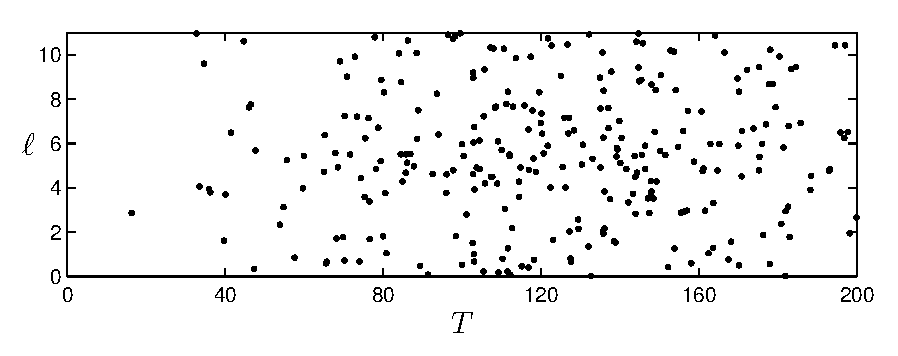
\includegraphics[width=0.7\textwidth]{figs/ks22_rpos_Tdelta.eps}
\end{center}
\caption{\Rpo s of \KSe\ with period $\period{}$ and phase shift $\shift$.
        } \label{f:ks22rposT}
\end{figure}

The largest Lyapunov exponent of \rpo s is shown in
\reffig{f:ks22rposL}.

\begin{figure}[t]
\begin{center}
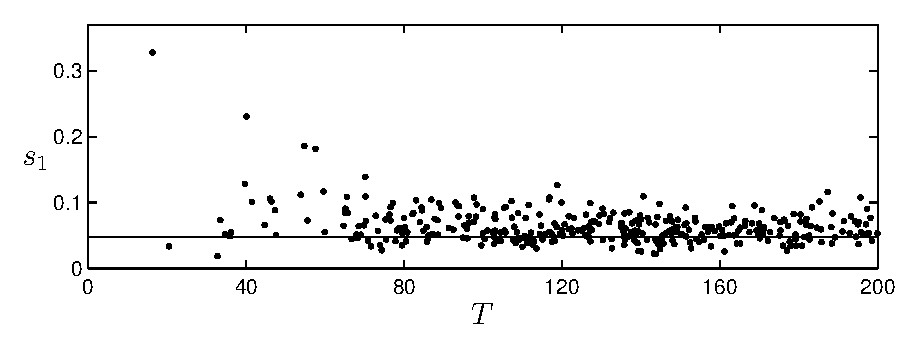
\includegraphics[width=0.7\textwidth]{figs/ks22_rpos_lyap.eps}
\end{center}
\caption{The largest Lyapunov exponent of \rpo s.
        } \label{f:ks22rposL}
\end{figure}

Next we describe several types of \rpo s.

\subsection{Short \rpo s}  The small period \rpo s outline the
coarse structure of the chaotic attractor, while the longer period
\rpo s typically just resolve the finer details of the dynamics
without significant modification of this structure.

The first five orbits with the shortest period we have found are
shown in \reffig{f:ks22rposShort}.  The shortest orbit with $\period{} =
16.4$ is also the most unstable, with one positive Lyapunov exponent
equal 0.328.  The other short orbits are less unstable, with the
largest Lyapunov exponents in the range 0.018 -- 0.073.  The
Lyapunov exponents of a \rpo are given by the formula
\[h_j = \log |\lambda_j|/\period{}\,,\]
where $\lambda_j$ are the eigenvalues of $g(\shift)J^T(a)$.  The
orbit with $\period{} = 20.5$ is exactly periodic due to a special symmetry
it possesses (see Section~\ref{ssec:po}).

\begin{figure}[t]
\begin{center}
\includegraphics[width=0.9\textwidth]{figs/ks22rposShort.eps}
%(a)\includegraphics[width=0.18\textwidth]{figs/ks22rpo016.3-02.86.eps}
%(b)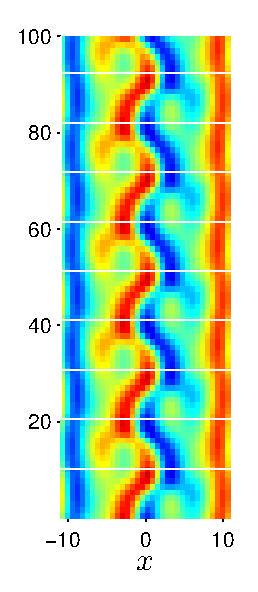
\includegraphics[width=0.18\textwidth]{figs/ks22rpo020.5-00.00.eps}
%(c)\includegraphics[width=0.18\textwidth]{figs/ks22rpo032.8-10.96.eps}
%(d)\includegraphics[width=0.18\textwidth]{figs/ks22rpo033.5-04.04.eps}
%(e)\includegraphics[width=0.18\textwidth]{figs/ks22rpo034.6-09.60.eps}
\end{center}
\caption{Short period \rpo s of \KS equation with $L = 22$: (a) $\period{} =
16.3$, $\shift = 2.86$; (b) $\period{} = 20.5$, $\shift = 0.00$ (periodic
orbit); (c) $\period{} = 32.8$, $\shift = 10.96$; (d) $\period{} = 33.5$, $\shift =
4.04$; (e) $\period{} = 34.6$, $\shift = 9.60$.  Horizontal and vertical
white lines indicate periodicity and phase shift of the orbits,
respectively. }\label{f:ks22rposShort}
\end{figure}


\subsection{\Rpo s close to the unstable manifold of \EQV{2} }
We have found a number of \rpo s which stay very close to the
unstable manifold of \EQV{2}.  This confirms that the "cage" of
unstable manifolds of equilibria plays an important role in
organizing the chaotic dynamics of \KS\ equation.

\begin{figure}[t]
\begin{center}
\includegraphics[width=0.9\textwidth]{figs/ks22rposCage.eps}
\end{center}
\caption{\Rpo s close to the unstable manifold of \EQV{2}
equilibrium. (a) $\period{} = 47.6$, $\shift = 5.68$; (b) $\period{} = 55.6$,
$\shift = 5.25$; (c) $\period{} = 59.9$, $\shift = 5.44$; (d) $\period{} = 71.7$,
$\shift = 5.503$; (e) $\period{} = 85.8$, $\shift = 5.503$. Horizontal and
vertical white lines indicate periodicity and phase shift of the
orbits, respectively. }\label{f:ks22rposCage}
\end{figure}

\subsection{Periodic Orbits} \label{ssec:po}
A \rpo\ will be eventualt periodic, i.e. $\shift = 0$, if it has one of
two symmetries: 1) $-u(-x,0) = u(x,0)$ or 2) $-u(-x,\period{}/2) =
u(x,0)$.\RLD{I have the feeling that it can be proven that there are
no other types of symmetries that lead to exactly periodic
solutions, but I don't know how to construct such a proof} In the
first case the whole orbit lives within the antisymmetric subspace.
The dynamics of \KS\ equation in the antisymmetric subspace has been
investigated in [include references]. The \KS\ equation with $L =
22$ appears not to have any periodic orbits of this type.
\RLD{Is it really
so?}

The second symmetry implies that the \rpo\ is reflection-\-sym\-metric
to itself after the time translation by half the period.

We have found 22 periodic orbits 
%(POs) 
with $\period{} < 200$.  The
shortest such orbit is shown in \reffig{f:ks22rposShort}(b).  Some
of the other periodic orbits are shown in \reffig{f:ks22rposPO}. Six
of the 22 \po s were found by the same method as used for locating
\rpo s, while the other orbits were found by directly employing the
symmetry of the \po:
\[ -u(-x+d,\period{}/2) = u(x,0)\,, \quad -L/2 < d \leq L/2\,.\]
In the Fourier space representation, this symmetry is expressed as
follows
\[
 -{\bf g}(d)a^\ast(\period{}/2) = a(0)\,.
\]
This condition is used to find a \po\ with period $\period{}$ (compare it to
the condition (\ref{eq:RPOcond}) for \rpo s). 
\RLD{
It looks like there
might be many more \po s than I initially expected to find. In fact, I
can even venture a guess that there are approximately as many \po s
with symmetry (2) within $\period{} < 200$ as there are \rpo s within $\period{} <
100$. The reasoning is that it shouldn't be any harder to match
$-u(-x+d,\period{}/2)$ and $u(x,0)$, than it is to match $u(x+d,\period{})$ and
$u(x,0)$, provided the dynamics is equally mixing for all types of
orbits.  If this is true, then the number of \po s with period smaller
than $\period{}/2$ should be approximately equal to the number of \rpo s with
period smaller than $\period{}$; the equality improving with increasing
$\period{}$.
    }


\begin{figure}[t] \label{f:ks22rposPO}
\begin{center}
\includegraphics[width=0.9\textwidth]{figs/ks22rposPO.eps}
\end{center}
\caption{
\Po s of \KS\ equation with $L = 22$: (a) $\period{} =
66.8$; (b) $\period{} = 87.2$; (c) $\period{} = 95.3$; (d) $\period{} = 96.4$; (e) $\period{} =
132.6$.
        }
\end{figure}

